% Options for packages loaded elsewhere
\PassOptionsToPackage{unicode}{hyperref}
\PassOptionsToPackage{hyphens}{url}
\PassOptionsToPackage{dvipsnames,svgnames,x11names}{xcolor}
%
\documentclass[
  letterpaper,
  DIV=11,
  numbers=noendperiod]{scrartcl}

\usepackage{amsmath,amssymb}
\usepackage{iftex}
\ifPDFTeX
  \usepackage[T1]{fontenc}
  \usepackage[utf8]{inputenc}
  \usepackage{textcomp} % provide euro and other symbols
\else % if luatex or xetex
  \usepackage{unicode-math}
  \defaultfontfeatures{Scale=MatchLowercase}
  \defaultfontfeatures[\rmfamily]{Ligatures=TeX,Scale=1}
\fi
\usepackage{lmodern}
\ifPDFTeX\else  
    % xetex/luatex font selection
\fi
% Use upquote if available, for straight quotes in verbatim environments
\IfFileExists{upquote.sty}{\usepackage{upquote}}{}
\IfFileExists{microtype.sty}{% use microtype if available
  \usepackage[]{microtype}
  \UseMicrotypeSet[protrusion]{basicmath} % disable protrusion for tt fonts
}{}
\makeatletter
\@ifundefined{KOMAClassName}{% if non-KOMA class
  \IfFileExists{parskip.sty}{%
    \usepackage{parskip}
  }{% else
    \setlength{\parindent}{0pt}
    \setlength{\parskip}{6pt plus 2pt minus 1pt}}
}{% if KOMA class
  \KOMAoptions{parskip=half}}
\makeatother
\usepackage{xcolor}
\setlength{\emergencystretch}{3em} % prevent overfull lines
\setcounter{secnumdepth}{-\maxdimen} % remove section numbering
% Make \paragraph and \subparagraph free-standing
\ifx\paragraph\undefined\else
  \let\oldparagraph\paragraph
  \renewcommand{\paragraph}[1]{\oldparagraph{#1}\mbox{}}
\fi
\ifx\subparagraph\undefined\else
  \let\oldsubparagraph\subparagraph
  \renewcommand{\subparagraph}[1]{\oldsubparagraph{#1}\mbox{}}
\fi

\usepackage{color}
\usepackage{fancyvrb}
\newcommand{\VerbBar}{|}
\newcommand{\VERB}{\Verb[commandchars=\\\{\}]}
\DefineVerbatimEnvironment{Highlighting}{Verbatim}{commandchars=\\\{\}}
% Add ',fontsize=\small' for more characters per line
\usepackage{framed}
\definecolor{shadecolor}{RGB}{241,243,245}
\newenvironment{Shaded}{\begin{snugshade}}{\end{snugshade}}
\newcommand{\AlertTok}[1]{\textcolor[rgb]{0.68,0.00,0.00}{#1}}
\newcommand{\AnnotationTok}[1]{\textcolor[rgb]{0.37,0.37,0.37}{#1}}
\newcommand{\AttributeTok}[1]{\textcolor[rgb]{0.40,0.45,0.13}{#1}}
\newcommand{\BaseNTok}[1]{\textcolor[rgb]{0.68,0.00,0.00}{#1}}
\newcommand{\BuiltInTok}[1]{\textcolor[rgb]{0.00,0.23,0.31}{#1}}
\newcommand{\CharTok}[1]{\textcolor[rgb]{0.13,0.47,0.30}{#1}}
\newcommand{\CommentTok}[1]{\textcolor[rgb]{0.37,0.37,0.37}{#1}}
\newcommand{\CommentVarTok}[1]{\textcolor[rgb]{0.37,0.37,0.37}{\textit{#1}}}
\newcommand{\ConstantTok}[1]{\textcolor[rgb]{0.56,0.35,0.01}{#1}}
\newcommand{\ControlFlowTok}[1]{\textcolor[rgb]{0.00,0.23,0.31}{#1}}
\newcommand{\DataTypeTok}[1]{\textcolor[rgb]{0.68,0.00,0.00}{#1}}
\newcommand{\DecValTok}[1]{\textcolor[rgb]{0.68,0.00,0.00}{#1}}
\newcommand{\DocumentationTok}[1]{\textcolor[rgb]{0.37,0.37,0.37}{\textit{#1}}}
\newcommand{\ErrorTok}[1]{\textcolor[rgb]{0.68,0.00,0.00}{#1}}
\newcommand{\ExtensionTok}[1]{\textcolor[rgb]{0.00,0.23,0.31}{#1}}
\newcommand{\FloatTok}[1]{\textcolor[rgb]{0.68,0.00,0.00}{#1}}
\newcommand{\FunctionTok}[1]{\textcolor[rgb]{0.28,0.35,0.67}{#1}}
\newcommand{\ImportTok}[1]{\textcolor[rgb]{0.00,0.46,0.62}{#1}}
\newcommand{\InformationTok}[1]{\textcolor[rgb]{0.37,0.37,0.37}{#1}}
\newcommand{\KeywordTok}[1]{\textcolor[rgb]{0.00,0.23,0.31}{#1}}
\newcommand{\NormalTok}[1]{\textcolor[rgb]{0.00,0.23,0.31}{#1}}
\newcommand{\OperatorTok}[1]{\textcolor[rgb]{0.37,0.37,0.37}{#1}}
\newcommand{\OtherTok}[1]{\textcolor[rgb]{0.00,0.23,0.31}{#1}}
\newcommand{\PreprocessorTok}[1]{\textcolor[rgb]{0.68,0.00,0.00}{#1}}
\newcommand{\RegionMarkerTok}[1]{\textcolor[rgb]{0.00,0.23,0.31}{#1}}
\newcommand{\SpecialCharTok}[1]{\textcolor[rgb]{0.37,0.37,0.37}{#1}}
\newcommand{\SpecialStringTok}[1]{\textcolor[rgb]{0.13,0.47,0.30}{#1}}
\newcommand{\StringTok}[1]{\textcolor[rgb]{0.13,0.47,0.30}{#1}}
\newcommand{\VariableTok}[1]{\textcolor[rgb]{0.07,0.07,0.07}{#1}}
\newcommand{\VerbatimStringTok}[1]{\textcolor[rgb]{0.13,0.47,0.30}{#1}}
\newcommand{\WarningTok}[1]{\textcolor[rgb]{0.37,0.37,0.37}{\textit{#1}}}

\providecommand{\tightlist}{%
  \setlength{\itemsep}{0pt}\setlength{\parskip}{0pt}}\usepackage{longtable,booktabs,array}
\usepackage{calc} % for calculating minipage widths
% Correct order of tables after \paragraph or \subparagraph
\usepackage{etoolbox}
\makeatletter
\patchcmd\longtable{\par}{\if@noskipsec\mbox{}\fi\par}{}{}
\makeatother
% Allow footnotes in longtable head/foot
\IfFileExists{footnotehyper.sty}{\usepackage{footnotehyper}}{\usepackage{footnote}}
\makesavenoteenv{longtable}
\usepackage{graphicx}
\makeatletter
\def\maxwidth{\ifdim\Gin@nat@width>\linewidth\linewidth\else\Gin@nat@width\fi}
\def\maxheight{\ifdim\Gin@nat@height>\textheight\textheight\else\Gin@nat@height\fi}
\makeatother
% Scale images if necessary, so that they will not overflow the page
% margins by default, and it is still possible to overwrite the defaults
% using explicit options in \includegraphics[width, height, ...]{}
\setkeys{Gin}{width=\maxwidth,height=\maxheight,keepaspectratio}
% Set default figure placement to htbp
\makeatletter
\def\fps@figure{htbp}
\makeatother

\KOMAoption{captions}{tableheading}
\makeatletter
\makeatother
\makeatletter
\makeatother
\makeatletter
\@ifpackageloaded{caption}{}{\usepackage{caption}}
\AtBeginDocument{%
\ifdefined\contentsname
  \renewcommand*\contentsname{Table of contents}
\else
  \newcommand\contentsname{Table of contents}
\fi
\ifdefined\listfigurename
  \renewcommand*\listfigurename{List of Figures}
\else
  \newcommand\listfigurename{List of Figures}
\fi
\ifdefined\listtablename
  \renewcommand*\listtablename{List of Tables}
\else
  \newcommand\listtablename{List of Tables}
\fi
\ifdefined\figurename
  \renewcommand*\figurename{Figure}
\else
  \newcommand\figurename{Figure}
\fi
\ifdefined\tablename
  \renewcommand*\tablename{Table}
\else
  \newcommand\tablename{Table}
\fi
}
\@ifpackageloaded{float}{}{\usepackage{float}}
\floatstyle{ruled}
\@ifundefined{c@chapter}{\newfloat{codelisting}{h}{lop}}{\newfloat{codelisting}{h}{lop}[chapter]}
\floatname{codelisting}{Listing}
\newcommand*\listoflistings{\listof{codelisting}{List of Listings}}
\makeatother
\makeatletter
\@ifpackageloaded{caption}{}{\usepackage{caption}}
\@ifpackageloaded{subcaption}{}{\usepackage{subcaption}}
\makeatother
\makeatletter
\@ifpackageloaded{tcolorbox}{}{\usepackage[skins,breakable]{tcolorbox}}
\makeatother
\makeatletter
\@ifundefined{shadecolor}{\definecolor{shadecolor}{rgb}{.97, .97, .97}}
\makeatother
\makeatletter
\makeatother
\makeatletter
\makeatother
\ifLuaTeX
  \usepackage{selnolig}  % disable illegal ligatures
\fi
\IfFileExists{bookmark.sty}{\usepackage{bookmark}}{\usepackage{hyperref}}
\IfFileExists{xurl.sty}{\usepackage{xurl}}{} % add URL line breaks if available
\urlstyle{same} % disable monospaced font for URLs
\hypersetup{
  pdftitle={One-way ANOVA using Python},
  pdfauthor={Isaac Ajao},
  colorlinks=true,
  linkcolor={blue},
  filecolor={Maroon},
  citecolor={Blue},
  urlcolor={Blue},
  pdfcreator={LaTeX via pandoc}}

\title{One-way ANOVA using Python}
\author{Isaac Ajao}
\date{2024-10-07}

\begin{document}
\maketitle
\ifdefined\Shaded\renewenvironment{Shaded}{\begin{tcolorbox}[breakable, boxrule=0pt, sharp corners, interior hidden, borderline west={3pt}{0pt}{shadecolor}, enhanced, frame hidden]}{\end{tcolorbox}}\fi

In this blog, we'll explore how to perform a One-Way ANOVA in Python to
compare the means of multiple groups and assess if they are
statistically different.

\hypertarget{introduction-to-one-way-anova-in-python}{%
\subsubsection{Introduction to One-Way ANOVA in
Python}\label{introduction-to-one-way-anova-in-python}}

When analyzing data, one of the key tasks is to determine whether the
means of different groups are significantly different from one another.
One powerful statistical test to help with this is the \textbf{Analysis
of Variance (ANOVA)}, specifically the \textbf{One-Way ANOVA}. This
technique is used when you have one independent categorical variable and
want to compare the means of two or more groups on a continuous
dependent variable.

\textbf{One-Way ANOVA} tests the null hypothesis that the means of
several groups are equal, versus the alternative hypothesis that at
least one group mean is different. It's particularly useful when dealing
with experiments or observational studies that involve comparisons
across multiple groups or categories.

In Python, we can easily perform One-Way ANOVA using libraries like
\textbf{SciPy} and \textbf{Statsmodels}, which offer user-friendly
methods for statistical analysis. In this tutorial, we will walk through
the steps of carrying out a One-Way ANOVA in Python, from setting up the
data to interpreting the results.

\hypertarget{when-to-use-one-way-anova}{%
\subsubsection{When to Use One-Way
ANOVA:}\label{when-to-use-one-way-anova}}

\begin{itemize}
\item
  You have \textbf{one categorical independent variable} with two or
  more groups (e.g., treatment types or different locations).
\item
  The dependent variable is \textbf{continuous} (e.g., height, weight,
  test scores).
\item
  The data should meet assumptions such as normality within each group
  and homogeneity of variances.
\end{itemize}

In the following sections, we will use Python to:

\begin{enumerate}
\def\labelenumi{\arabic{enumi}.}
\item
  Set up and explore the data.
\item
  Perform One-Way ANOVA using \texttt{scipy.stats} and
  \texttt{statsmodels}.
\item
  Interpret the ANOVA results and check assumptions.
\end{enumerate}

\hypertarget{load-the-necessary-libraries}{%
\subsubsection{Load the necessary
libraries}\label{load-the-necessary-libraries}}

\begin{Shaded}
\begin{Highlighting}[]
\CommentTok{\# Load the necessary libraries}
\ImportTok{import}\NormalTok{ pandas }\ImportTok{as}\NormalTok{ pd}
\ImportTok{from}\NormalTok{ scipy }\ImportTok{import}\NormalTok{ stats}
\ImportTok{import}\NormalTok{ statsmodels.api }\ImportTok{as}\NormalTok{ sm }\CommentTok{\# for statistical analysis}
\ImportTok{from}\NormalTok{ statsmodels.formula.api }\ImportTok{import}\NormalTok{ ols }\CommentTok{\# for statistical analysis}
\ImportTok{import}\NormalTok{ seaborn }\ImportTok{as}\NormalTok{ sns }\CommentTok{\# to plot charts }
\ImportTok{import}\NormalTok{ matplotlib.pyplot }\ImportTok{as}\NormalTok{ plt }\CommentTok{\# to plot charts}
\end{Highlighting}
\end{Shaded}

\begin{Shaded}
\begin{Highlighting}[]
\CommentTok{\# Data setup}
\NormalTok{data }\OperatorTok{=}\NormalTok{ \{}
    \StringTok{\textquotesingle{}Group\textquotesingle{}}\NormalTok{: [}\StringTok{\textquotesingle{}Group 1\textquotesingle{}}\NormalTok{, }\StringTok{\textquotesingle{}Group 2\textquotesingle{}}\NormalTok{, }\StringTok{\textquotesingle{}Group 3\textquotesingle{}}\NormalTok{, }\StringTok{\textquotesingle{}Group 4\textquotesingle{}}\NormalTok{] }\OperatorTok{*} \DecValTok{3}\NormalTok{,}
    \StringTok{\textquotesingle{}Layout\textquotesingle{}}\NormalTok{: [}\StringTok{\textquotesingle{}A\textquotesingle{}}\NormalTok{] }\OperatorTok{*} \DecValTok{4} \OperatorTok{+}\NormalTok{ [}\StringTok{\textquotesingle{}B\textquotesingle{}}\NormalTok{] }\OperatorTok{*} \DecValTok{4} \OperatorTok{+}\NormalTok{ [}\StringTok{\textquotesingle{}C\textquotesingle{}}\NormalTok{] }\OperatorTok{*} \DecValTok{4}\NormalTok{,}
    \StringTok{\textquotesingle{}Time\_Spent\textquotesingle{}}\NormalTok{: [}\DecValTok{12}\NormalTok{, }\DecValTok{14}\NormalTok{, }\DecValTok{11}\NormalTok{, }\DecValTok{13}\NormalTok{, }\DecValTok{15}\NormalTok{, }\DecValTok{18}\NormalTok{, }\DecValTok{14}\NormalTok{, }\DecValTok{17}\NormalTok{, }\DecValTok{10}\NormalTok{, }\DecValTok{13}\NormalTok{, }\DecValTok{12}\NormalTok{, }\DecValTok{11}\NormalTok{]}
\NormalTok{\}}

\NormalTok{df }\OperatorTok{=}\NormalTok{ pd.DataFrame(data)}
\BuiltInTok{print}\NormalTok{(}\StringTok{"}\CharTok{\textbackslash{}n}\StringTok{Data on time spent}\CharTok{\textbackslash{}n}\StringTok{"}\NormalTok{, df)}
\end{Highlighting}
\end{Shaded}

\begin{verbatim}

Data on time spent
       Group Layout  Time_Spent
0   Group 1      A          12
1   Group 2      A          14
2   Group 3      A          11
3   Group 4      A          13
4   Group 1      B          15
5   Group 2      B          18
6   Group 3      B          14
7   Group 4      B          17
8   Group 1      C          10
9   Group 2      C          13
10  Group 3      C          12
11  Group 4      C          11
\end{verbatim}

\begin{Shaded}
\begin{Highlighting}[]
\CommentTok{\# Performing one{-}way ANOVA}
\NormalTok{model }\OperatorTok{=}\NormalTok{ ols(}\StringTok{\textquotesingle{}Time\_Spent \textasciitilde{} C(Layout)\textquotesingle{}}\NormalTok{, data }\OperatorTok{=}\NormalTok{ df).fit()}
\NormalTok{anova\_table }\OperatorTok{=}\NormalTok{ sm.stats.anova\_lm(model,typ}\OperatorTok{=}\DecValTok{2}\NormalTok{)}
\end{Highlighting}
\end{Shaded}

\begin{Shaded}
\begin{Highlighting}[]
\CommentTok{\# Printing the ANOVA table}
\BuiltInTok{print}\NormalTok{(anova\_table)   }\CommentTok{\# reject Ho (null hypothesis) if p{-}value is less than 0.05 which says there\textquotesingle{}s no diff in means in the groups}

\BuiltInTok{print}\NormalTok{(model.summary())}
\end{Highlighting}
\end{Shaded}

\begin{verbatim}
              sum_sq   df      F    PR(>F)
C(Layout)  44.666667  2.0  10.05  0.005088
Residual   20.000000  9.0    NaN       NaN
                            OLS Regression Results                            
==============================================================================
Dep. Variable:             Time_Spent   R-squared:                       0.691
Model:                            OLS   Adj. R-squared:                  0.622
Method:                 Least Squares   F-statistic:                     10.05
Date:                Mon, 14 Oct 2024   Prob (F-statistic):            0.00509
Time:                        13:43:17   Log-Likelihood:                -20.092
No. Observations:                  12   AIC:                             46.18
Df Residuals:                       9   BIC:                             47.64
Df Model:                           2                                         
Covariance Type:            nonrobust                                         
==================================================================================
                     coef    std err          t      P>|t|      [0.025      0.975]
----------------------------------------------------------------------------------
Intercept         12.5000      0.745     16.771      0.000      10.814      14.186
C(Layout)[T.B]     3.5000      1.054      3.320      0.009       1.115       5.885
C(Layout)[T.C]    -1.0000      1.054     -0.949      0.368      -3.385       1.385
==============================================================================
Omnibus:                        2.312   Durbin-Watson:                   3.525
Prob(Omnibus):                  0.315   Jarque-Bera (JB):                0.932
Skew:                          -0.000   Prob(JB):                        0.628
Kurtosis:                       1.635   Cond. No.                         3.73
==============================================================================

Notes:
[1] Standard Errors assume that the covariance matrix of the errors is correctly specified.
\end{verbatim}

\begin{verbatim}
C:\Users\user\AppData\Local\Programs\Python\Python311\Lib\site-packages\scipy\stats\_axis_nan_policy.py:418: UserWarning: `kurtosistest` p-value may be inaccurate with fewer than 20 observations; only n=12 observations were given.
  return hypotest_fun_in(*args, **kwds)
\end{verbatim}

\begin{Shaded}
\begin{Highlighting}[]
\CommentTok{\# Post{-}hoc test (Tukey\textquotesingle{}s HSD)}
\ImportTok{from}\NormalTok{ statsmodels.stats.multicomp }\ImportTok{import}\NormalTok{ pairwise\_tukeyhsd}

\NormalTok{tukey }\OperatorTok{=}\NormalTok{ pairwise\_tukeyhsd(endog}\OperatorTok{=}\NormalTok{df[}\StringTok{\textquotesingle{}Time\_Spent\textquotesingle{}}\NormalTok{], groups}\OperatorTok{=}\NormalTok{df[}\StringTok{\textquotesingle{}Layout\textquotesingle{}}\NormalTok{], alpha}\OperatorTok{=}\FloatTok{0.05}\NormalTok{)}
\BuiltInTok{print}\NormalTok{(tukey)}
\end{Highlighting}
\end{Shaded}

\begin{verbatim}
Multiple Comparison of Means - Tukey HSD, FWER=0.05
==================================================
group1 group2 meandiff p-adj  lower  upper  reject
--------------------------------------------------
     A      B      3.5  0.022  0.557  6.443   True
     A      C     -1.0 0.6251 -3.943  1.943  False
     B      C     -4.5 0.0053 -7.443 -1.557   True
--------------------------------------------------
\end{verbatim}

\begin{Shaded}
\begin{Highlighting}[]
\CommentTok{\# Visualizing the results}
\NormalTok{sns.boxplot(x}\OperatorTok{=}\StringTok{\textquotesingle{}Layout\textquotesingle{}}\NormalTok{, y}\OperatorTok{=}\StringTok{\textquotesingle{}Time\_Spent\textquotesingle{}}\NormalTok{, data}\OperatorTok{=}\NormalTok{df)}
\NormalTok{plt.title(}\StringTok{\textquotesingle{}User Engagement Time by Website layout\textquotesingle{}}\NormalTok{)}
\NormalTok{plt.xlabel(}\StringTok{\textquotesingle{}Website layout\textquotesingle{}}\NormalTok{)}
\NormalTok{plt.ylabel(}\StringTok{\textquotesingle{}Time Spent (minute)\textquotesingle{}}\NormalTok{)}
\NormalTok{plt.show()}
\end{Highlighting}
\end{Shaded}

\begin{figure}[H]

{\centering 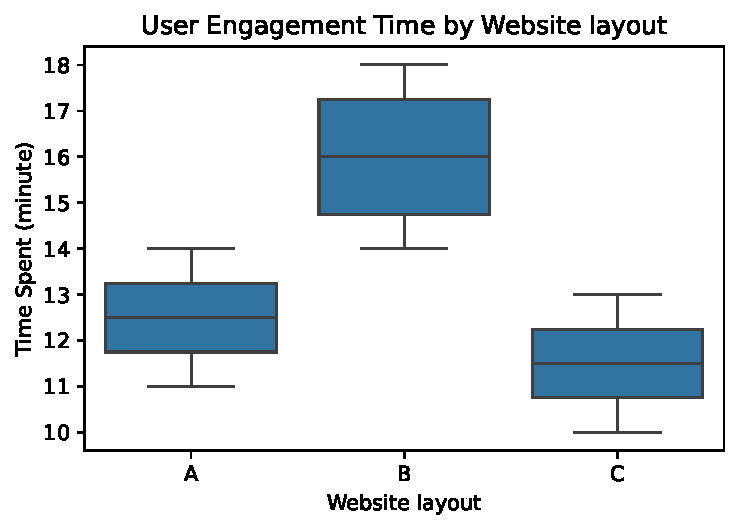
\includegraphics{one-way-anova_files/figure-pdf/cell-7-output-1.pdf}

}

\end{figure}

\hypertarget{resources}{%
\subsection{Resources}\label{resources}}

You can also watch \texttt{One-way\ Anova\ using\ Python} on my YouTube
channel for details:

\url{https://www.youtube.com/watch?v=UCDW5wvVBB8\&t=88s}

\begin{center}\rule{0.5\linewidth}{0.5pt}\end{center}



\end{document}
